\chapter{面向问题复述识别的定向数据增强方法}

上一章采用多粒度卷积交互推理方法强化了模型对“问题与答案”之间的精细语义感知能力,其有利于优化问答场景下相关答案的召回质量。
本章集中研究问题复述识别任务中“问题与问题”之间的精细语义关系,用以提高问答场景下同义问题(已知答案)的召回精度。
% 该任务旨在召回“同质异构”的问句对子(语义相同表述迥异的问句),
% 其可被降解为面向自然问句的二元分类问题,即对输入的问句对子进行“复述”和“非复述”的二相判别。
现有预训练语言模型被广泛应用于自然语言的语义编码,并取得了显著的性能优势。
然而,其优势并未在问题复述的求解中得到充分的体现,原因在于:
1)预训练语言模型善于生成通用的语义表示,对特定任务中精细的语义表示需求并不敏感;
2)复述样本的“是与非”往往取决于极为微妙的语义差异。
微调预训练语言模型成为提高其任务适应性的关键步骤,但其极大依赖训练数据的数量(多样性)与质量(可靠性)。
为此,本章提出一种基于生成模型的定向数据增强方法(DDA)。
该方法能够利用诱导标签对神经生成网络进行引导,借以自动生成多样的复述和非复述的增强样本,促进训练数据的自动扩展。
此外,本章设计了一种多模型集成的标签投票机制,并用其修正增强样本的潜在标签错误,以此提高扩展数据的可靠性。
在中文问题复述数据集LCQMC上的实验结果证明,与传统数据增强方案相比,本章方法生成的样本质量更高,且语义表达更加多元化。
下面将详细介绍本章的研究动机、相关方法以及具体的实验论证。

\section{引言}

问题复述识别是问答匹配研究领域中的重要任务之一,
其旨在判断两个自然问句的语义是否等价或具有较高相似度,即对输入的问句对子进行“复述”和“非复述”的二相判别。
如表~\ref{table4-1}~中{\kai“移动号码如何转为电信号码?”}与{\kai“能把移动转为电信号码吗?”},这两个问句表达的意思完全相同,为复述关系(标签为1表示复述关系)。
当前,问题复述识别技术已经被广泛应用到多种实际场景中,如:搜索引擎、社区问答以及智能客服等。
深度神经网络的发展推动了复述识别等自然语言处理(Natural Language Processing,简称NLP)的研究。
其中,BERT\cite{devlin2018bert}等基于大规模语料预训练的语言模型能够复用并微调其注意力和联合编码机制,
使其具有适应性更强的文本语义特征提取和交互能力,在问题复述识别等任务中表现出色。

\begin{table}[h]
    \caption{LCQMC及增强数据示例}
    \centering
    \newcommand{\tabincell}[2]{\begin{tabular}{@{}#1@{}}#2\end{tabular}}
    \begin{tabular}{lllcc}
    \toprule[0.7pt]
    \textbf{样本来源} & \textbf{问题1} & \textbf{问题2}& \textbf{标签}& \textbf{合格?} \\
    \midrule[0.7pt]

    LCQMC & \multirow{4}{*}{移动号码如何转为电信号码?} & 能把移动转为电信号码吗? & 1 & Y \\
    BT & & 如何将手机号码转换为电信号码? & 1 & N \\
    EDA &  & 移动号码转为电信号码? & 1 & Y \\
    DDA &  & 电信号码可以改为移动号码吗? & 0 & Y \\
    \midrule[0.4pt]
    LCQMC & \multirow{4}{*}{什么牌子空调最好?} & 什么牌子空调扇最好? & 0 & Y \\
    BT &  & 哪个牌子的空调最好? & 1 & Y \\
    EDA &  & 什么牌子的空气调节最好? & 1 & N \\
    DDA &  & 空调什么牌子最好? & 1 & Y \\


    \bottomrule[0.7pt]
    \end{tabular}
    \label{table4-1}
\end{table}

现代神经网络模型在训练过程中往往需要大量的标注数据进行学习。
但是,标注给定句子的复述句需要消耗庞大的人力成本,这导致了当前的复述识别数据集往往规模有限。
这种普遍的数据稀缺性问题对模型的泛化性和鲁棒性提出了极大的挑战。
当前,数据增强策略(Data Augmentation)是扩充数据样本规模的一种有效方法,在一定程度上能够缓解数据因素对模型学习能力的制约。
Wei等提出简单数据增强策略EDA\cite{wei2019eda},
其在原始样本的基础上采用随机删除、插入、交换、同义词替换四种操作构造增强样本。
Yu等采用的回译策略BT\cite{yu2018qanet}将英文样本翻译为法文,然后再翻译回英文,
期望样本在保持原意的前提下能够增加、删除、修改原词或重新组织原句。
如表~\ref{table4-1}~所示(Y表示样本质量合格,N表示样本质量不合格),尽管EDA和BT策略能够高效地扩充数据数量,但是其仅能构造与原样本语义相同的数据,
并且无法保证构造样本的语法正确性和标签一致性(即样本不合格),这些包含错误知识的数据对模型产生负面影响。

本章提出一种基于生成模型的定向数据增强策略(Directional Data Augmentation,简称DDA),
在预训练语言模型UNILM(Unified Language Model)\cite{bao2020unilmv2}的输入中添加定向标签,使其生成期望的复述句或非复述句。
UNILM强大的生成能力能有效降低文本的语法错误率。
此外,为了进一步提高数据质量,确保问题对的标签真实性,本章设计了一种标签修正策略,对新生成的文本对的标签进行纠错。
从表~\ref{table4-1}~可以看出,相比于EDA等方案,UNILM语言模型产出的样本质量更高,样本难度更大。
同时,DDA策略仅使用定向标签约束生成样本的语义,使其具有多元化变动,更加符合真实语言环境,有助于提高模型的鲁棒性。
本章在LCQMC\cite{liu2018lcqmc}中文问题复述数据集上进行实验,并在多个基线模型上验证DDA策略的有效性。
本章的主要贡献有:

\begin{enumerate}
    \item 
    提出一种通用的定向数据增强方案,能够大规模地产出高质量、多元化的“复述”与“非复述”的数据样本。
    \item 
    基于中文问题复述语料LCQMC构造公开增强数据集LCQMC$_{DDA}$,实验表明其对基线模型的性能及泛化能力具有普遍的提升作用。
\end{enumerate}

本章的组织形式如下:第1节为引言部分;第2节详细介绍本章所提出的定向数据增强方法;第3节对方法进行实验验证及分析;第4节总结本章并展望未来工作。


\section{系统框架及主要研究内容}

\subsection{总体结构}

数据规模与质量对于模型的学习过程往往起到至关重要的作用。尤其在小规模数据集上,数据增强策略能够为模型带来巨大收益。
本章基于UNILM语言模型生成定向增强样本,同时采用多判别器集成投票策略修正样本标签,最终形成高质量的问题复述识别样本。

\subsection{定向问题生成}

本章使用LCQMC数据训练定向问题生成模型。
LCQMC中的样本是由问题$Q$、问题$Q^t$以及标签$L$三者组成的三元组$(Q,Q^t,L)$,
其中$L\in\{0,1\}$表示$Q$与$Q^t$是否为复述关系。
本章使用预训练语言模型UNILM构建定向问题生成模型。
UNILM在BERT的自编码MLM(Masked Language Model)\cite{taylor1953cloze}任务基础上,
加入部分自回归的掩码策略,使得模型不仅具有捕获上下文语义能力,
而且能够对连续的掩码部分进行整体预测,增强模型词块、词组的理解和生成能力。

传统的问题复述生成模型利用某一给定源问题$Q$,生成与源问题语义一致的复述问句$Q^\prime$。
本章提出的定向问题生成策略,在输入中加入定向引导标签$L\in\{0,1\}$,
使其引导模型在不同语义方向上对问句做微小改动,强化模型的定向生成能力。
当$L=1$时,期望生成与源问题$Q$语义一致的复述问题$Q^\prime$;
当$L=0$时,期望生成与源问题$Q$语义不一致,但两者之间字面高度相似的非复述问题$Q^\prime$,
使得问题复述判别模型容易将$Q$与$Q^\prime$误判为语义一致的复述问题对。
最终,生成模型的输入如下:
\begin{equation}
    X=\{[CLS],L,[SEP],Q,[SEP]\} \notag
\end{equation}
其中,$[CLS]$是包含整个输入部分语义信息的标志,$[SEP]$是用以区分输入中多个成分的分隔符号。
UNILM将$X$的特征表示输入多层双向Transformer\cite{vaswani2017attention}编码块构成的编码器,
从而得到问题$Q$和定向引导标签$L$的联合编码表示$T$:
\begin{equation}
    T=\{T_{[CLS]},T_{[L]},T_{[SEP]},T_{[Q]},T_{[SEP]}\} \notag
\end{equation}
值得说明的是,Transformer含有多头自注意力机制。
因此,联合编码表示$T$中的分布特征已经得到注意力加权,
此时,$T_{[Q]}$中已经充分融合了定向标签$L$的特征信息。
最终,将联合编码表示$T$作为生成目标问句$Q^\prime$的隐状态逐步生成目标问句$Q^\prime$,
将其与真实目标问句$Q^t$进行拟合,其损失计算公式如下:
\begin{equation}
    \mathcal{L}_G({q_i}^\prime)=-logP({q_i}^\prime\ =\ {q_i}^t\ |\  L,Q,{q_{<i}}^t,{q_i}^\prime)
\end{equation}
其中,$\mathcal{L}_G$表示负对数似然损失。
${q_i}^\prime$和${q_i}^t$分别是生成的目标问题$Q^\prime$与真实目标问句$Q^t$中第$i$个词。

通过上述训练方式,模型在生成时能捕获到定向诱导标签、源问题以及目标问题当前时间步之前的信息,
使得模型在预测阶段能够参考定向诱导标签生成期望的复述或非复述问句。
如表~\ref{table4-1}~所示,源问题为{\kai“什么牌子空调最好?”},
当给定诱导标签$L\ =\ 1$时,模型可定向生成与源问题语义一致的问句{\kai“空调什么牌子最好?”};
当给定源问题{\kai“移动号码如何转为电信号码?”}及定向诱导标签$L\ =\ 0$时,
模型可生成与源问题语义不同却字面相似的问句{\kai“电信号码如何转为移动号码?”}。

本章使用LCQMC复述数据集进行实验,利用模型生成一批与原样本标签相反的增强数据。
本章将LCQMC三元组$(Q,Q^t,L)$中的源问题$Q$以及标签的反置$!L$(当$L=0$时,$!L=1$;当$L=1$时,$!L=0$)作为定向生成模型的输入,从而得到新的增强样本$(Q,Q^\prime,!L)$。
最终,本章在LCQMC的23.8万样本的基础上,扩充了一批标签相反的增强样本,
经过简单的规则过滤(剔除$Q^\prime$与$Q$完全一致或过于相近的样本),共保留16.3万条有效样本。

\subsection{标签修正}

定向生成模型能够将定向诱导标签和问句的特征表达相融合,生成语义与诱导标签走向一致的目标问句。
本章仅采用定向标签进行语义诱导,其包含的信息内容简单,对模型限制的较少且使用代价微小,使模型生成的问句更加具有多样性。
但由于没有更多的外部知识引导定向问题的语义特征,这种方法导致增强样本中仍存在一些不满足定向诱导标签语义要求的问句。
例如,表~\ref{table4-4}~中的源问题{\kai“长方体的底面积怎么求?”},给定诱导标签$1$时,模型生成的问句{\kai“长方体的面积怎么求?”}语义已经发生偏转,该样本实际上是标签为$0$的非复述样本。
因此,本章采用人工标注方法,从增强样本中标注出1,000条作为增强样本测试集,用以验证增强样本的标签与人工标注标签的一致率,
标注结果显示样本标签一致率为70.2\%。

对此,本章设计了一种基于多判别模型的集成投票方法,用以修正增强样本的标签。
本章使用BERT$_{base}$\cite{devlin2018bert}、RoBERTa$_{large}$\cite{liu2019roberta}和MacBERT$_{large}$\cite{cui2020revisiting}三种预训练语言模型在LCQMC数据集上进行微调,以此作为问题复述判别器基线。
本章将源问题$Q$以及目标问题$Q^t$作为判别器的输入,预测两者之间是否为复述关系$L^\prime$,
并将其与真实标签$L$进行拟合。具体的损失计算公式如下:
\begin{equation}
    \mathcal{L}_D(L,L^\prime)=-Llog(p)-(1-L)log(1-p)
\end{equation}
其中,$\mathcal{L}_D$表示二分类交叉熵损失,$p$为样本为复述关系的概率。
本章使用以上三个判别器对源问题$Q$与生成的目标问题$Q^\prime$进行预测,
若两个或两个以上模型预测结果与定向标签相符合,则将定向标签作为最终标签。
否则,将三个模型预测的复述概率均值$p>=\alpha$的样本修正为复述问题对,即标签为1;
将复述概率均值$p<=\beta$的样本修正为非复述问题对,即标签为0($score\in[0,1]$)。
通过在LCQMC$_{DDA}$测试集合上不断调试(详见~\ref{4.3.3 标签修正策略分析}~节),
本章发现当$\alpha$取值0.92且$\beta$取值0.5时,修正后的样本标签与$L’$人工标注的标签最为接近,
标签一致率约95\%,共将约3.1万条样本修正为复述样本,9千条样本修正为非复述样本。
本章将标签修正后的16.3万条样本作为增强数据集LCQMC$_{DDA}$,用于优化问题复述识别模型在目标数据集上的性能以及鲁棒性。


\section{实验及结果分析}

\subsection{数据集与评价方法}

本章在中文问题复述数据集LCQMC上进行实验,验证DDA方法的有效性,数据集的详细介绍见~\ref{2.2 语料资源概述}~小节。
本章提出的DDA数据增强策略,针对LCQMC数据集构造了对应的增强数据集LCQMC$_{DDA}$。
其样本格式与LCQMC完全一致,共包含约16.5万个问题对。
表~\ref{table4-2}~列出了LCQMC$_{DDA}$增强数据集的统计信息。
本章实验采用准确率Acc评价模型的二元分类能力,具体介绍见~\ref{2.3 性能评价指标}~小节。

\begin{table}
    \caption{LCQMC$_{DDA}$数据统计表}
    \centering
    \newcommand{\tabincell}[2]{\begin{tabular}{@{}#1@{}}#2\end{tabular}}
    \begin{tabular}{l|l|l|l}
    \toprule[0.7pt]
    & \;\textbf{总计} & \;\textbf{正样本} & \;\textbf{负样本} \\
    \midrule[0.7pt]

    训练集\quad\; & \;163,158\; & \;68,968\; & \;94,190 \\
    测试集 & \;1,000 & \;465 & \;535 \\
    \bottomrule[0.7pt]
    \end{tabular}
    \label{table4-2}
\end{table}

\subsection{基线模型与超参设置}

\textbf{(一) 定向问题生成模型}

本章基于UNILM(v2)模型架构(12-layer,768-hidden,12-heads)进行微调。
UNILM(v2)采用部分自回归的掩码策略,使模型能对连续的mask部分进行整体预测,增加了模型对词块的理解和生成能力。
输入的源问句与目标问句最大长度限制均为35。
模型在训练阶段batch\_size设置为64,优化函数的学习率(leraning\_rate)设置为2e-5,
优化函数中的epsilon\cite{rutherford2002lecture}设置为1e-8。

\textbf{(一) 问题复述判别模型}

本章使用BERT$_{base}$、RoBERTa$_{large}$和MacBERT$_{large}$三种预训练语言模型作为问题复述识别任务的判别模型:
\begin{itemize}
    \item \textbf{BERT$_{base}$}(Devlin et al., 2018)\cite{devlin2018bert}
    使用Transformer作为主要架构,能更彻底的捕获文本中的双向关系。
    其在海量语料上使用语言掩码任务(Mask Lanauage Model)以及句对预测任务(Next Sentence Prediction)
    进行自监督训练,学习蕴含上下文的动态特征表达。
    \item \textbf{RoBERTa$_{large}$}(Liu et al., 2019)\cite{liu2019roberta}
    对比BERT模型而言,其参数量、语料规模更大,并且采用动态掩码策略使训练语料的利用的更加充分,在NLP任务中的表现更加出色。
    \item \textbf{MacBERT$_{large}$}(Rutherford et al., 2020)\cite{cui2020revisiting}
    是在RoBERTa基础上改进的中文语言模型,其借助近义词工具(Synonyms)\footnote{https://github.com/chatopera/Synonyms}获取掩码词的近义词或同义词进行替换,
    能够缓解预训练与微调(fine-tune)阶段的误差,以及提高模型的鲁棒性。
\end{itemize}

本章判别模型输入问题对的最大长度限制为65。模型在训练阶段batch\_size设置为64,优化器的学习率设置为5e-6,
优化函数中的epsilon设置为1e-8。

\subsection{定向数据增强(DDA)实验分析}

为了验证本章方法的有效性,本章将LCQMC$_{DDA}$作为增强数据扩充到LCQMC数据集中,并将其对判别模型的增强结果进行分析。
本章通过数据增强技术探索DDA策略对这些基线模型的作用。
此外,为了从多种角度评判DDA策略为问题复述识别模型带来的泛化性及鲁棒性综合收益,
本章还在公开的问题复述鲁棒性评测数据CQM$_{robust}$(详见章节\ref{5.point3})上进行评估。
相较于传统数据集,CQM$_{robust}$中蕴含多种中文语言特征,且样本迷惑性较强,对判别模型的挑战更大。并且该测试集中的样本均来源于百度搜索中的真实问题,与真实世界中的样本分布更接近。
因此,其实验结果更能反映DDA策略产出数据的真实性和多样性。

\begin{table}
    \caption{DDA数据增强试验结果}
    \centering
    \newcommand{\tabincell}[2]{\begin{tabular}{@{}#1@{}}#2\end{tabular}}
    \begin{tabular}{l|l|cc|c|c}
    \toprule[0.7pt]
    \multirow{2}{*}{\textbf{模型}} & \multirow{2}{*}{\enspace \textbf{训练数据\enspace }} & \multicolumn{2}{c|}{\textbf{LCQMC}} & \;\textbf{LCQMC$_{DDA}$}\; & \;\textbf{CQM$_{robust}$}\; \\
    \cline{3-6}
    & & \enspace Dev\; & \; Test\enspace & Test & Test\\
    \midrule[0.7pt]

    \multirow{3}{*}{BERT$_{base}$} & \enspace LCQMC & 89.1 & 86.5 & 83.5 & 71.6 \\\cline{2-6}
    &\enspace + DDA$_{noise}$ & 84.7 & 83.4 & 77.4 & 70.6 \\
    &\enspace \textbf{+ DDA} & \textbf{90.2} & \textbf{87.7} & \textbf{86.9} & \textbf{74.4} \\
    \midrule[0.4pt]
    \multirow{2}{*}{RoBERTa$_{large}$} & \enspace LCQMC & 90.5 & 88.0 & 84.6 & 75.9 \\
    &\enspace \textbf{+ DDA} & \textbf{90.9} & \textbf{88.6} & \textbf{87.2} & \textbf{77.8} \\
    \midrule[0.4pt]
    \multirow{2}{*}{MacBERT$_{large}$\quad} & \enspace LCQMC & 90.9 & 88.2 & 84.6 & 78.0 \\
    &\enspace \textbf{+ DDA} & \textbf{91.2} & \textbf{89.5} & \textbf{87.0} & \textbf{79.2} \\
    \bottomrule[0.7pt]
    \end{tabular}
    \label{table4-3}
\end{table}

表~\ref{table4-3}~列出了上述判别模型在数据增强前后的实验结果。
由表可知,DDA增强数据不仅提高了模型在LCQMC测试数据上的表现,也增强了模型应对领域外复杂样本的能力,
其在CQM$_{robust}$上的性能平均提升了约2\%。
此外,在基线模型中,MacBERT针对中文特点进行相似词掩码间接优化模型泛化能力,因此其在基线中的性能最高。
尽管如此,本章通过DDA策略对其强化训练后,MacBERT的准确率仍有平均近1.3\%的提升。
实验结果表明,本章所提DDA数据增强方案对测试集在所有基线上的表现均有提升作用,其数据增强样本具有较强的普适性和多样性。

\begin{table}
    \caption{LCQMC$_{DDA}$数据样例}
    \centering
    \newcommand{\tabincell}[2]{\begin{tabular}{@{}#1@{}}#2\end{tabular}}
    \begin{tabular}{llc}
    \toprule[0.7pt]
    \textbf{问题1} &  \textbf{问题2} & \textbf{标签} \\
    \midrule[0.7pt]

    怎么养仓鼠? & 仓鼠怎么养?& 1 \\
    \midrule[0.4pt]
    公分跟厘米一样吗? & 公分就是厘米吗? & 1\\
    \midrule[0.4pt]
    长方体的底面积怎么求? & 长方体的面积怎么求? &  0 \\
    \midrule[0.4pt]
    现在农村种什么最赚钱?\quad\; & 现在农村做什么最赚钱?\;\; & 0 \\
    \bottomrule[0.7pt]
    \end{tabular}
    \label{table4-4}
\end{table}

值得注意的是,基线模型在LCQMC$_{DDA}$测试数据上的准确率比在LCQMC上低,这表明DDA方式构造的增强数据样本难度更大。
如表~\ref{table4-4}~所示,LCQMC$_{DDA}$中包含更多迷惑性较强的样本,对提升模型的鲁棒性有较大帮助。
本章对此进行了详细分析。表~\ref{table4-5}~展示了基线模型在LCQMC$_{DDA}$测试集合上的详细准确率。
显而易见,模型在正样本(复述样本)上的表现远高于在负样本(非复述样本)上的表现,负样本的准确率平均低于正样本28.5\%,由此说明DDA数据增强策略生成的负样本难度更大。
从表~\ref{table4-4}~中例子可以明显看出LCQMC$_{DDA}$中的负样本比正样本更加具有迷惑性。本文猜测这一现象与定向生成任务的特性相关。

定向生成任务通过给定诱导标签,对源问句的特征表达加以扰动,从而生成期望的复述或非复述关系的目标问句。
尽管在生成模型中加入的定向诱导标签可以使源问句的语义发生迁移,但是该诱导标签中包含的信息量过于单一(0或1标签),目标问句中仍保留有绝大部分的源问句信息,从而导致目标问句与源问句的字面倾向于相似。
因此,最终构造的复述关系增强样本整体偏简单,非复述关系增强样本整体迷惑性更高。
这种现象导致了模型更容易识别出LCQMC$_{DDA}$中的复述样本,更容易对字面相似的非复述样本作出误判。


\begin{table}
    \caption{LCQMC$_{DDA}$详细性能}
    \centering
    \newcommand{\tabincell}[2]{\begin{tabular}{@{}#1@{}}#2\end{tabular}}
    \begin{tabular}{l|c|c}
    \toprule[0.7pt]
    \textbf{模型} &  \enspace \textbf{正样本} \enspace& \enspace \textbf{负样本} \\
    \midrule[0.7pt]

    BERT$_{base}$ & 97.9 &  \enspace 66.9 \\
    RoBERTa$_{large}$ & 97.9 &  \enspace 69.3 \\
    MacBERT$_{large}$\quad\; & 96.7 &  \enspace 70.8 \\

    \bottomrule[0.7pt]
    \end{tabular}
    \label{table4-5}
\end{table}

本章统计了LCQMC$_{DDA}$中所有问题对的编辑距离分布,结果如图~\ref{fig4-1}~所示,70\%以上的目标问句与源问句之间的编辑距离小于或等于5。
由此说明,大量生成的负样本能满足与源问题字面相似的要求,使其最终构成问题对具有较高的迷惑性,从而导致模型容易产生错误。

\begin{figure}
    \centering
      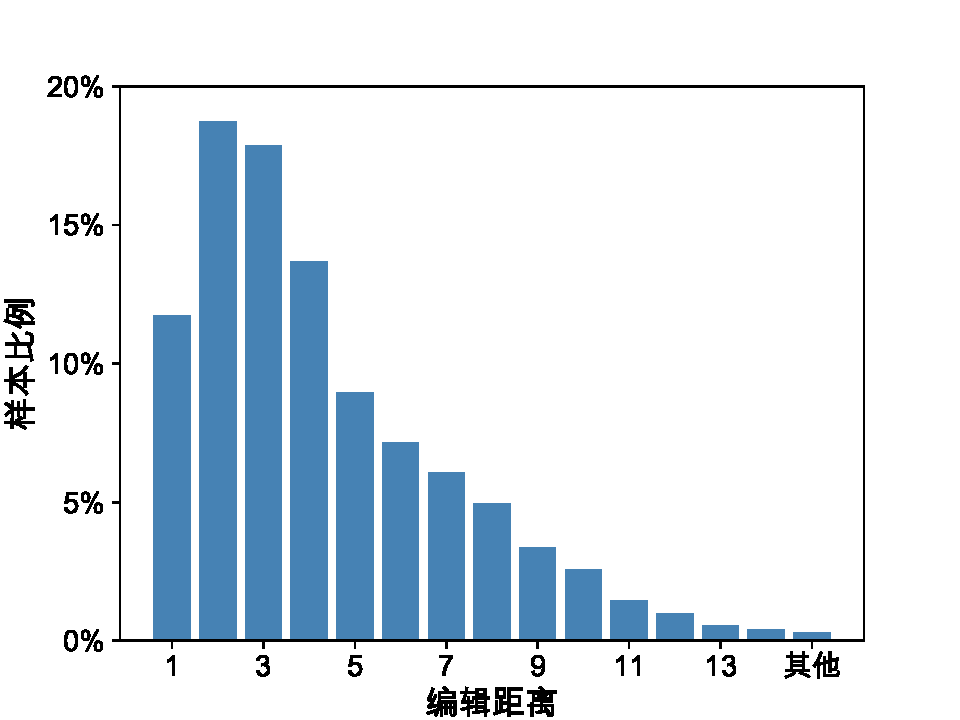
\includegraphics[scale=0.5]{figure/fig4-1.pdf}
    \caption{LCQMC$_{DDA}$数据编辑距离统计}
    \label{fig4-1}
\end{figure}

\subsection{标签修正策略分析}\label{4.3.3 标签修正策略分析}

本节使用上述三个基线判别模型集成投票的方式修正样本的定向诱导标签。
若多票($>=2$)与定向标签一致,则保留定向标签为样本最终标签;
否则,将预测结果为复述关系的概率均值$p$作为标签判断依据。
若$p>=\alpha$,则将定向标签为0的样本修正为标签为1的正样本;
若$p<=\beta$,则将定向标签为1的样本修正为标签为0的负样本。
借助LCQMC$_{DDA}$人工标注的测试集可统计出标签修正的准确度,
表~\ref{table4-6}~和表~\ref{table4-7}~分别展示了$\alpha$和$\beta$取值对正负样本修正准确度的影响。
其中,“修正”表示修正后的标签与人工评估标签一致;
“误修正”表示修正后的标签与人工评估标签不一致;“净修正”是两者差值。

\begin{table}
    \caption{正样本标签阈值统计表}
    \centering
    \newcommand{\tabincell}[2]{\begin{tabular}{@{}#1@{}}#2\end{tabular}}
    \begin{tabular}{l|c|c|c}
    \toprule[0.7pt]
    \textbf{$\alpha$\qquad\enspace  } &  \enspace\textbf{修正}  \enspace&  \;\textbf{误修正} \; & \enspace \textbf{净修正} \\
    \midrule[0.7pt]

    0.95 & 144 & 12 & \enspace 132\\
    \textbf{0.92} & \textbf{161} & \textbf{17} & \enspace \textbf{144}\\
    0.8 & 173 &  41 & \enspace 132\\
    0.7 & 182 &  51 & \enspace 131\\
    0.6 & 188 &  59 & \enspace 129\\
    0.5 & 192 &  71 & \enspace 121\\

    \bottomrule[0.7pt]
    \end{tabular}
    \label{table4-6}
\end{table}

由表可见,当$\alpha=0.92$时,将负样本修正为正样本的净修正量最多;
当$\beta=0.5$时,将正样本修正为负样本的净修正量最多。
由于DDA策略构造的负样本具有一定的迷惑性,所以模型预测负样本为复述关系的概率整体偏高,即$\beta$的取值偏高。
最终,本章使用该阈值对16.3万条训练样本进行标签修正,共将31,596条样本修正为正样本,9,140条样本修正为负样本。
本章对标签修正前后的训练数据进行了数据增强对比实验,在BERT$_{base}$基线上的结果如表~\ref{table4-3}~所示,标签修正后的数据(+DDA)比未修正的数据(+DDA$_{noise}$)在增强训练后的准确率平均提升约5.8\%。

\begin{table}
    \caption{负样本标签阈值统计表}
    \centering
    \newcommand{\tabincell}[2]{\begin{tabular}{@{}#1@{}}#2\end{tabular}}
    \begin{tabular}{l|c|c|c}
    \toprule[0.7pt]
    \textbf{$\beta$\qquad\enspace } &   \enspace \textbf{修正}  \enspace& \; \textbf{误修正} \;&  \enspace \textbf{净修正} \\
    \midrule[0.7pt]

    0.1 & 37 & 0 & \enspace 37 \\
    0.2 & 49 & 1 & \enspace 48 \\
    0.3 & 60 & 2 & \enspace 58 \\
    0.4 & 72 & 4 & \enspace 68 \\
    \textbf{0.5} & \textbf{78} & \textbf{5} & \enspace \textbf{73} \\

    \bottomrule[0.7pt]
    \end{tabular}
    \label{table4-7}
\end{table}

\subsection{训练集规模实验分析}

模型在较小的数据集上进行训练时,过拟合现象往往更为严重。
为了探究DDA对于不同规模数据的增强效果,本章将LCQMC的数据分割为不同大小的子集,
其数据量分别为:$\{4w,\ 8w,\ 12w,\ 16w,20w,ALL\}$(ALL表示LCQMC全部数据)。
本章在不同规模的子集上对BERT$_{base}$进行DDA数据增强实验,并在LCQMC测试集上评估其准确率。

\begin{figure}[h]
    \centering
      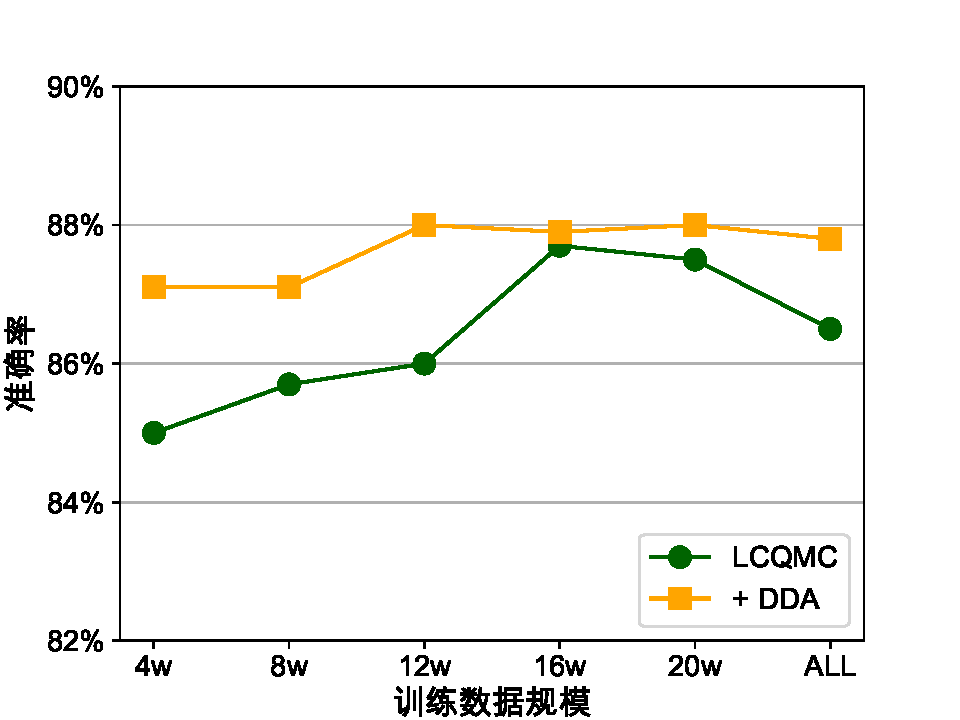
\includegraphics[scale=0.5]{figure/fig4-2.pdf}
    \caption{LCQMC测试集性能曲线}
    \label{fig4-2}
\end{figure}

如图~\ref{fig4-2}~所示,当训练数据量较小时,DDA策略与基线的差异更加明显,这表明DDA对规模较小的数据集效果更为显著。
此外,从图中可以明显看出,当LCQMC的数据量增大到16万后,基线模型逐渐出现过拟合现象,继续增加数据量性能反而有下降趋势。
反观DDA数据增强策略,其性能曲线并未随着数据量的增加有明显下降趋势。
DDA增强数据中包含一些难度较大、具有迷惑性的样本,能够有效提高神经网络模型的泛化能力和鲁棒性,抑制过拟合现象的产生。

\subsection{显著性分析}

本章使用显著性检验确保实验结果并非偶然结果,即重复进行了多次实验(5次)计算使用DDA数据增强策略前后,基线在各个测试集上准确率指标的P-value值。
由表~\ref{table4-8}~可见,本章所提出的DDA数据增强方法在多个基线上的不同测试集结果P-value值均小于0.05,即均存在显著提升。

\begin{table}[h]
    \caption{显著性分析结果}
    \centering
    \newcommand{\tabincell}[2]{\begin{tabular}{@{}#1@{}}#2\end{tabular}}
    \begin{tabular}{l|c|c|c}
    \toprule[0.7pt]
    \textbf{模型} & \enspace\textbf{LCQMC}\enspace & \enspace\textbf{LCQMC$_{DDA}$}\enspace & \enspace\textbf{CQM$_{robust}$} \\
    \midrule[0.7pt]

    BERT$_{base}$   & 3.4e-3 & 8.7e-4 & \enspace 5.2e-4 \\
    RoBERTa$_{large}$ & 4.2e-2 & 1.3e-3 & \enspace 4.1e-3 \\
    MacBERT$_{large}$\quad\quad & 1.3e-3 & 1.9e-2 & \enspace 3.2e-3 \\

    \bottomrule[0.7pt]
    \end{tabular}
    \label{table4-8}
\end{table}

\section{本章小结}

本章提出了一种面向问题复述识别任务的定向数据增强策略DDA,该方法可以定向构造蕴含精细语义的高质量样本,促进训练数据的自动扩展。
实验结果表明DDA能够有效提高问题复述识别模型的鲁棒性与泛化能力。
然而,本章并未对模型性能提升的细节展开进一步的实验分析与探究,从而无法精确衡量模型优化前后的能力差异。
% 然而,本章对于模型鲁棒性提升的细节尚未展开进一步的探究。
因此,下一章将基于中文语法特征对问题复述识别模型进行系统化的评估,深入分析模型具体能力及其鲁棒性的变化。
% 在未来的工作中,我们将进一步提高定向生成环节的样本质量,以及对标签修正环节进行优化。
% 同时,尝试将该方法应用到其他NLP领域中。